\documentclass[xcolor={table,usenames,dvipsnames}]{article}
\usepackage{float}
\usepackage[french]{babel}
\setlength{\parindent}{0pt}
\setlength{\parskip}{6pt}  % Adds spacing between paragraphs
\usepackage{ccicons}
\usepackage{caption}
\captionsetup{justification=centering}
\usepackage{tcolorbox} % For the title box
\usepackage{xcolor}    % For colors
\usepackage{graphicx}  % For inserting images
\usepackage{listings}
\definecolor{mygray}{rgb}{0.8,0.8,0.8}
\lstset{%
	basicstyle=\ttfamily,
	breaklines = true,
	backgroundcolor=\color{mygray},
}
\usepackage{realboxes}

\DeclareDocumentCommand{\clist}{v}{%
	\Colorbox{mygray}{\csname lstinline\endcsname!#1!}%
}

\definecolor{BlueViolet}{RGB}{5, 9, 141} % Define the missing BlueViolet color
\usepackage{hyperref}  % For clickable Table of Contents
 \hypersetup{
	colorlinks=true,      % Enable colored links
	linkcolor=violet,        % Color for internal links (sections, equations, etc.)
	citecolor=BlueViolet,      % Color for citations
	filecolor=magenta,    % Color for file links
	urlcolor=BlueViolet         % Color for URLs
}





\let\oldnocite\nocite
\makeatletter
\renewcommand*{\nocite}[1]{\oldnocite{#1}\Hy@backout{#1}}
\makeatother



\usepackage[style=authoryear, maxbibnames=99, mincitenames=1, maxcitenames=2, backref=true, hyperref=true, dashed=false, firstinits=true, backend=bibtex, bibencoding=utf8, uniquename=false, uniquelist=false, natbib=true]{biblatex}
\renewcommand*{\bibfont}{\scriptsize}

% Remove quotation marks from titles
\DeclareFieldFormat[article,incollection,inproceedings,conference]{title}{#1} 

% Define a custom color for the title box
\definecolor{myblue}{RGB}{44, 62, 80}

\addbibresource{bibliographie.bib} 

\author{Ljudmila PETKOVI\'C}
\title{\textbf{\textsc{M2SOL034} Corpus, ressources et linguistique outillée}}

\begin{document}
	
	% Insert the logo at the top (centered)
	\begin{center}
		
\includegraphics[width=3cm]{img/logo.png} % Adjust width as needed
	\end{center}
	
	% Create a rectangle around the title
	\begin{tcolorbox}[colback=myblue!10, colframe=myblue, width=\textwidth, sharp corners, boxrule=1pt]
		\centering
		\Large \textbf{\textsc{M2SOL034} Corpus, ressources et linguistique outillée\\{\large\textsc{TD 4} : \texttt{Unitex}}}
	\end{tcolorbox}
	
	\begin{center}
		Ljudmila PETKOVI\'C
		
		{\small Sorbonne Université\\Master \og{}Langue et Informatique\fg{} (\textsc{M1} ScLan)\\\textsc{UFR} Sociologie et Informatique pour les Sciences Humaines\\Semestre 2, 2024-2025, le \today}
	\end{center}
	


		
	% Hyperlinked Table of Contents
	\tableofcontents
	
	\bigskip
	
\section{Exercices}
	Les exercices suivants sont à faire sur le corpus \textit{Tour du monde en 80 jours} de Jules Verne.
\begin{enumerate}
	\item \textbf{Manipulation de graphe}
	\begin{itemize}
		\item compléter le graphe \texttt{je,tu,il...} pour qu'il reconnaisse un pronom personnel suivi d'un verbe (n'importe lequel, sous n'importe quelle forme)
		\item l'appliquer sur le texte
	\end{itemize}
	\\
	\bigskip
	
\item \textbf{Recherches de motifs complexes}
	\begin{itemize}
		\item toutes les occurrences des pronoms personnels (\textit{je, tu, il$\dots$})
		\item toutes les occurrences des pronoms personnels qui sont suivis par un verbe
		\item toutes les suites de 3 adjectifs (\texttt{A}) : qu'observez-vous de surprenant ?
%		\item toutes les suites de noms. Pourquoi le motif \texttt{<N>*} produit-il une erreur ? Que faire pour l'éviter ?
	\end{itemize}
	\\
	\bigskip
	
	\item \textbf{Recherches utilisant les informations grammaticales|flexionnelles|sémantiques}
	\begin{itemize}
		\item tous les adjectifs au féminin pluriel
		\item tous les mots possédant le trait sémantique \og{}humain collectif\fg{}
		\item tous les verbes à l'imparfait du langage courant
	\end{itemize}
	
		\\
	\bigskip
	
	\item \textbf{Recherches complexes utilisant la concaténation et l'union}
	\begin{itemize}
		\item tous les verbes, soit à l'imparfait, soit au présent ou à l'imparfait du subjonctif
	\end{itemize}
	\\
	\bigskip

\item \textbf{Recherches utilisant les négations}
\begin{itemize}
\item tous les mots qui ne sont pas dans le dictionnaire
\item tous les mots qui ne sont pas écrits tout en minuscules
\item tous les noms non humains
\end{itemize}
	\\
\bigskip

\item \textbf{Recherches à l'aide de métamotifs}
\begin{itemize}
	\item tous les mots commençant par une majuscule
	\item tous les mots qui possèdent le trait sémantique \og{}concret\fg{}
\end{itemize}
\\
\bigskip

\item \textbf{Recherches utilisant les filtres}
\begin{itemize}
	\item tous les mots qui commencent par \textit{anti} ou \textit{pro}, suivis par un tiret facultatif
	\item tous les mots composés contenant un tiret
	\item tous les mots qui ne sont pas dans le dictionnaire et qui se terminent par \textit{es}
\end{itemize}
\\
\bigskip
 
 \item \textbf{Regex avancées}
 \begin{itemize}
 	\item tous les verbes un peu ou très spécialisés, soit au participe passé, soit à l'infinitif
 	\item toutes les séquences
 	\begin{itemize}
 		\item commençant par le verbe \textit{avoir}, et
 		\item se terminant par un verbe au participe passé
 	\end{itemize}
 	\item tous les verbes au subjonctif passé ou présent, contenant \textit{uiss}
 \end{itemize}
\\
\bigskip
\item \textbf{Transformer le texte}

Créer un graphe qui réalise un début d'anonymisation du \textit{Tour du monde en 80 jours}
	\begin{itemize}
	\item remplacer toutes les occurrences de \textit{Phileas Fogg} par \texttt{Pers1}
	\item remplacer toutes les occurrences de \textit{Passepartout} par \texttt{Pers2}
	\item l'appliquer sur le texte et vérifier les résultats obtenus
\end{itemize}

\\
\bigskip


\item \textbf{Annoter le texte}

Créer un graphe qui réalise un début d'annotation en entités nommées du \textit{Tour de monde en 80 jours}
	\begin{itemize}
	\item annoter toutes les occurrences de \textit{Phileas Fogg} et de \textit{Passepartout} par des balises \texttt{<pers></pers>}
	\item appliquer le graphe sur le texte et vérifier les résultats obtenus
\end{itemize}
\end{enumerate}






\section{Solutions}

\begin{enumerate}
	\item 
	Repérage des pronoms personnels suivis d'un verbe (Fig. \ref{fig:jetuil}).
	
	\texttt{je+tu+il+elle+on+nous+vous+ils+elles <V>}
	
			\begin{figure}[H] % Use [H] to force the figure to stay in place
		\centering
		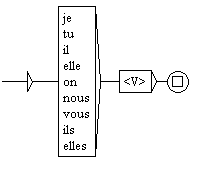
\includegraphics[width=.3\linewidth]{img/jetuil.png}
		\caption{Repérage des pronoms personnels suivis d'un verbe.}
		\label{fig:jetuil}
	\end{figure}
	
	\item Repérage des pronoms personnels avec une seule balise, suivis d'un verbe (Fig. \ref{fig:jetuil_balise}).
		\begin{figure}[H] % Use [H] to force the figure to stay in place
		\centering
		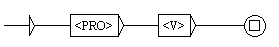
\includegraphics[width=1\linewidth]{img/pronom_verbe.png}
		\caption{Repérage des pronoms avec une seule balise, suivis d'un verbe.}
		\label{fig:jetuil_balise}
	\end{figure}
	
	Repérage des suites d'au moins 3 adjectifs (\texttt{A}).
			\begin{figure}[H] % Use [H] to force the figure to stay in place
		\centering
		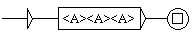
\includegraphics[width=.7\linewidth]{img/adjectifs.png}
		\caption{Repérage des suites de trois adjectifs.}
		\label{fig:jetuil_balise}
	\end{figure}
	
	Nous remarquons également le repérage de certains faux positifs dans le résultat du concordancier (adverbes, locutions$\dots$).
	
	\bigskip
	\item Repérage de tous les adjectifs au féminin pluriel (Fig. \ref{fig:adjectif_fp}).
		\begin{figure}[H] % Use [H] to force the figure to stay in place
		\centering
		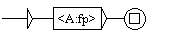
\includegraphics[width=.7\linewidth]{img/adjectif_fp.png}
		\caption{Repérage des adjectifs au féminin pluriel.}
		\label{fig:adjectif_fp}
	\end{figure}
	
	\\
	\bigskip
	
		 Repérage de tous les noms possédant le trait sémantique \og{}humain collectif\fg{} (Fig. \ref{fig:collectif}).
	\begin{figure}[H] % Use [H] to force the figure to stay in place
		\centering
		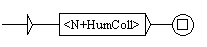
\includegraphics[width=.7\linewidth]{img/collectif.png}
		\caption{Repérage de tous les noms possédant le trait sémantique \og{}humain collectif\fg{}.}
		\label{fig:collectif}
	\end{figure}
	
	\\
	\bigskip
	
	Repérage des verbes à l'imparfait du langage courant (Fig. \ref{fig:verbe_impf}).
			\begin{figure}[H] % Use [H] to force the figure to stay in place
		\centering
		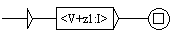
\includegraphics[width=.7\linewidth]{img/verbe_impf_courant.png}
		\caption{Repérage des verbes à l'imparfait du langage courant.}
		\label{fig:verbe_impf}
	\end{figure}
	
	\item Repérage de tous les verbes, soit à l'imparfait, soit au présent ou à l'imparfait du subjonctif (Fig. \ref{fig:verbe_impf_pres_impfsubj}).
				\begin{figure}[H] % Use [H] to force the figure to stay in place
		\centering
		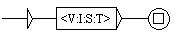
\includegraphics[width=.7\linewidth]{img/verbe_impf_pres_impfsubj.png}
		\caption{Repérage de tous les verbes, soit à l'imparfait, soit au présent ou à l'imparfait du subjonctif.}
		\label{fig:verbe_impf_pres_impfsubj}
	\end{figure}
	
		\bigskip
	\\
	\item Repérage de tous les mots qui ne sont pas dans le dictionnaire (Fig. \ref{fig:dic}).
					\begin{figure}[H] % Use [H] to force the figure to stay in place
		\centering
		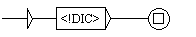
\includegraphics[width=.7\linewidth]{img/dic.png}
		\caption{Repérage des mots hors dictionnaire.}
		\label{fig:dic}
	\end{figure}
	
	\bigskip
	\\
	
	Repérage de tous les mots qui ne sont pas écrits tout en minuscules (Fig. \ref{fig:min}).
						\begin{figure}[H] % Use [H] to force the figure to stay in place
		\centering
		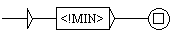
\includegraphics[width=.7\linewidth]{img/min.png}
		\caption{Repérage de tous les mots qui ne sont pas écrits tout en minuscules.}
		\label{fig:min}
	\end{figure}
	
	\bigskip
	\\
	
	Repérage de tous les noms non humains (Fig. \ref{fig:negation}).
							\begin{figure}[H] % Use [H] to force the figure to stay in place
		\centering
		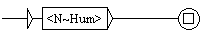
\includegraphics[width=.7\linewidth]{img/negation.png}
		\caption{Repérage de tous les mots non humains.}
		\label{fig:negation}
	\end{figure}
	
	\item Repérage de tous les mots commençant par une majuscule à l'aide des métamotifs (Fig. \ref{fig:majuscule}).
		\begin{figure}[H] % Use [H] to force the figure to stay in place
		\centering
		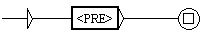
\includegraphics[width=.7\linewidth]{img/majuscule.png}
		\caption{Repérage de tous les mots commençant par une majuscule à l'aide des métamotifs.}
		\label{fig:majuscule}
	\end{figure}
	
	\bigskip
	\\
	Repérage de tous les mots qui possèdent le trait sémantique \og{}concret\fg{} (Fig. \ref{fig:concret}).
	\begin{figure}[H] % Use [H] to force the figure to stay in place
		\centering
		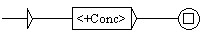
\includegraphics[width=.7\linewidth]{img/concret.png}
		\caption{Repérage de tous les mots qui possèdent le trait sémantique \og{}concret\fg{}.}
		\label{fig:concret}
	\end{figure}
		\bigskip
	\\
	
	\item Repérage de tous les mots qui commencent par \textit{anti} ou \textit{pro}, suivis par un tiret facultatif (Fig. \ref{fig:anti_pro}).
		\begin{figure}[H] % Use [H] to force the figure to stay in place
		\centering
		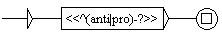
\includegraphics[width=.7\linewidth]{img/anti_pro.png}
		\caption{Repérage de tous les mots qui commencent par \textit{anti} ou \textit{pro}, suivis par un tiret facultatif.}
		\label{fig:anti_pro}
	\end{figure}
	\bigskip
	\\
	
		Repérage de tous les mots composés contenant un tiret (Fig. \ref{fig:composes}).
	\begin{figure}[H] % Use [H] to force the figure to stay in place
		\centering
		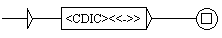
\includegraphics[width=.7\linewidth]{img/composes.png}
		\caption{Repérage de tous les mots composés contenant un tiret.}
		\label{fig:composes}
	\end{figure}
	\bigskip
	\\
	
			Repérage de tous les mots qui ne sont pas dans le dictionnaire et qui se terminent par \textit{es} (Fig. \ref{fig:es}).
	\begin{figure}[H] % Use [H] to force the figure to stay in place
		\centering
		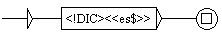
\includegraphics[width=.7\linewidth]{img/es.png}
		\caption{Repérage de tous les mots qui ne sont pas dans le dictionnaire et qui se terminent par \textit{es}.}
		\label{fig:es}
	\end{figure}
	
	\bigskip
	\\
	\item Repérage de tous les verbes un peu ou très spécialisés, soit au participe passé, soit à l'infinitif (Fig. \ref{fig:specialises}).
			\begin{figure}[H] % Use [H] to force the figure to stay in place
		\centering
		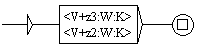
\includegraphics[width=.7\linewidth]{img/specialises.png}
		\caption{Repérage de tous les verbes un peu ou très spécialisés, soit au participe passé, soit à l'infinitif.}
		\label{fig:specialises}
	\end{figure}
	
	\bigskip
	\\
	
	Repérage de toutes les séquences commençant par le verbe \textit{avoir} et se terminant par un verbe au participe passé (Fig. \ref{fig:participe_passe}).
	\begin{figure}[H] % Use [H] to force the figure to stay in place
		\centering
		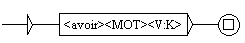
\includegraphics[width=.7\linewidth]{img/participe_passe.png}
		\caption{Repérage de toutes les séquences commençant par le verbe \textit{avoir} et se terminant par un verbe au participe passé.}
		\label{fig:participe_passe}
	\end{figure}
	
	\bigskip
	\\
	Repérage de tous les verbes au subjonctif passé ou présent, contenant \textit{uiss} (Fig. \ref{fig:uiss}).
	\begin{figure}[H] % Use [H] to force the figure to stay in place
		\centering
		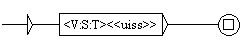
\includegraphics[width=.7\linewidth]{img/uiss.png}
		\caption{Repérage de tous les verbes au subjonctif passé ou présent, contenant \textit{uiss}.}
		\label{fig:uiss}
	\end{figure}
	
	\item Remplacer toutes les occurrences de \textit{Phileas Fogg} par \texttt{Pers1} et de \textit{Passepartout} par \textit{Pers2} (Fig. \ref{fig:pers1_2}).
		\begin{figure}[H] % Use [H] to force the figure to stay in place
		\centering
		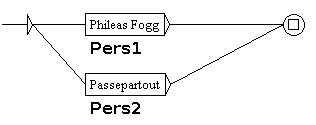
\includegraphics[width=.7\linewidth]{img/pers1_2.png}
		\caption{Remplacer toutes les occurrences de \textit{Phileas Fogg} par \texttt{Pers1} et de \textit{Passepartout} par \textit{Pers2}.}
		\label{fig:pers1_2}
	\end{figure}
		\bigskip
	\\
	
	\item Annoter toutes les occurrences de \textit{Phileas Fogg} et de \textit{Passepartout} par des balises \texttt{<pers></pers>} (Fig. {\ref{fig:pers}).
				\begin{figure}[H] % Use [H] to force the figure to stay in place
			\centering
			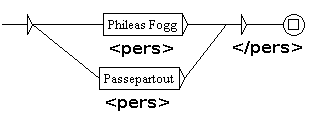
\includegraphics[width=.7\linewidth]{img/pers.png}
			\caption{Annoter toutes les occurrences de \textit{Phileas Fogg} et de \textit{Passepartout} par des balises \texttt{<pers></pers>}.}
			\label{fig:pers}
		\end{figure}
\end{enumerate}
\hline 

		\printbibliography


	\centering
{\small Le contenu de cette présentation est sous licence \texttt{CC-BY-NC-SA 4.0}\\Utilisation non commerciale -- Partage dans les mêmes conditions.\\}
\href{https://creativecommons.org/licenses/by-nc-sa/4.0/deed.fr}{\ccbyncsa}
	
\end{document}
